\section{Problem Description} \label{sec:problem_description}
    
    The concept of multi-hop reasoning presupposes a knowledge graph (KG) whose nodes (entities) and edges (relations) can be traversed via a chain of inference steps. In our setting, this KG is encoded in \emph{textual} form, but structurally, we are still dealing with \emph{multi-hop question answering} over a KG (Multi-hop KGQA). Prior work \citep{liu_joint_2022} has already observed that \emph{knowledge graph completion} can be critical for multi-hop KGQA; for \emph{grokking}-based Transformer generalization circuits to form, it becomes \emph{imperative} to extend the original KG such that sufficiently many multi-step (inferred) facts exist. This section formalizes our problem of \emph{augmenting} a KG to enable Transformer grokking.
    
    \subsection{Definitions and Basics} \label{subsec:definitions_basics}
        
        We begin by introducing key notations for clarity. Readers can refer to Table~\ref{tab:key_notation} at any time for a concise summary of the main symbols.
        
        \paragraph{Knowledge Graph.}
            \begin{definition}[Knowledge Graph]
                \label{def:kg}
                We define a knowledge graph as a tuple 
                \(
                    \mathcal{KG} = (\mathcal{V}, \mathcal{R}, \mathcal{F}_A),
                \)
                where
                \begin{itemize}
                    \item \(\mathcal{V}\) is a finite set of \textbf{entities} (nodes or vertices),
                    \item \(\mathcal{R}\) is a finite set of \textbf{relation types} (edges/predicates),
                    \item \(\mathcal{E} \equiv \mathcal{F}_A \subseteq \mathcal{V} \times \mathcal{R} \times \mathcal{V}\) 
                          is a finite set of \textbf{atomic facts} (triplets) of the form 
                          \((h,r,t)\), where \(h \in \mathcal{V}\) is a \emph{head} (subject), 
                          \(t \in \mathcal{V}\) is a \emph{tail} (object), and \(r \in \mathcal{R}\) is the relation.
                \end{itemize}
            \end{definition}
        
            In natural language, entities are typically connected by relational statements. Although some relations (e.g., ``son of'') are directed, one can also treat the KG as undirected for \emph{graph traversal} since a statement is often queryable in both directions (subject/object).
        
            \begin{definition}[Norm over edges]
                \label{def:norm_over_edges}
                For counting strictly \emph{directed} edges in \(\mathcal{KG}\) \emph{as if} they were undirected, we use the trivial count:
                \(|\;| = \sum_{(h, \dots, t) \in \mathcal{E}} 1.\)
                %\[
                %    || = \sum_{(h,\dots,t)\in \mathcal{E}} 1.
                %\]
                %For counting edges in \emph{as if} they were undirected, see Appendix \ref{sec:appendix_edgeNorm}.
            \end{definition}
        
            \begin{definition}[Average branching factor]
                \label{def:branching_factor}
                The \emph{average branching factor} of a knowledge graph is:
                \(b = \frac{|\mathcal{F}_A|}{|\mathcal{V}|}\).
                %\[
                    %b = \frac{|\mathcal{F}_A|}{|\mathcal{V}|}
                    %\quad\text{or}\quad
                    %b_U = \frac{|\mathcal{F}_A|_U}{|\mathcal{V}|}
                    %\quad(\text{undirected case}).
                %\]
            \end{definition}
            
            \begin{definition}[Atomic Facts]
                \label{def:atomic_facts}
                Following prior work, we use \(\mathcal{F}_A\) (or equivalently \(\mathcal{F}_1\)) to denote the set of \textbf{atomic facts}, i.e., all \textbf{first-order} triplets explicitly stored in the knowledge graph.
            \end{definition}
        
            \begin{example}[Running Example: Basic KG]
                \label{ex:basics_KG}
                Consider the KG in Figure~\ref{fig:exampleGraph} with
                \[
                \begin{aligned}
                    &\mathcal{V} = \{\text{``Obama''}, \text{``Michelle''}, 
                                     \text{``1964''}, \text{``Mary Poppins''}\}, \\
                    &\mathcal{R} = \{\text{``wife of''}, \text{``born in''}, 
                                     \text{``aired in''}\}.
                \end{aligned}
                \]
                The atomic facts \(\mathcal{F}_A\) include:
                \[
                \begin{aligned}
                    &\bigl(\text{``Michelle''}, \text{``wife of''}, \text{``Obama''}\bigr), \\
                    &\bigl(\text{``Michelle''}, \text{``born in''}, \text{``1964''}\bigr), \\
                    &\bigl(\text{``Mary Poppins''}, \text{``aired in''}, \text{``1964''}\bigr).
                \end{aligned}
                \]
                Hence, 
                \(\mathcal{F}_1 = \mathcal{F}_A\).
                The average branching factor here is \(b = 0.75\).
            \end{example}

            %\rule{\linewidth}{0.5pt} %0.5pt line for reference
        
            \begin{figure}[ht]
                \centering
                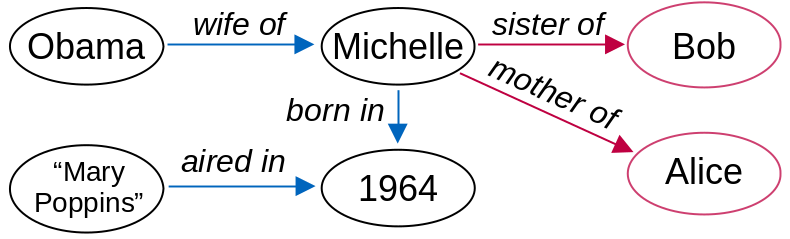
\includegraphics[width=0.4\textwidth, trim=0cm 0cm 0cm 0cm, clip]{exampleGraph_reduced.png}
                \caption{
                    \textbf{Exemplary Knowledge Graph with Synthesized Data.} Four original nodes (\textbf{black}) and three relations (\textbf{blue}) result in two inferred facts. Two additional synthetic nodes and relations (\textbf{red}) extend the amount of inferred facts by four. Consequently, $\phi_I=\phi_2$ increases from $\frac{2}{3}\approx0.66$ to $\frac{6}{5}=1.2$.
                }
                \label{fig:exampleGraph}
            \end{figure}
            
        
        \paragraph{Inference Steps and Paths.}
            \begin{definition}[Inference Step]
                \label{def:inference_step}
                An inference step is a function
                \(I: \mathcal{V} \times \mathcal{R} \to \mathcal{V}\)
                that traverses the graph from one entity to a neighboring entity via one relation:
                \[
                    I(h, r) = t
                    \quad\text{where}\quad
                    (h,r,t) \in \mathcal{F}_A.
                \]
            \end{definition}
        
            \begin{definition}[Inference Path]
                \label{def:inference_path}
                An inference path \(p_n\) of length \(n\) is a sequence of relations 
                \(p_n = (r_1, \dots, r_n) \in \mathcal{R}^n\).
                The path is \textbf{simple} if each relation leads to exactly one successor node (no branching ambiguity):
                \begin{align*}
                    \forall r_i \in p_n\ :\ &\exists v_{i-1}, v_i \in \mathcal{V} \text{ such that } I(v_{i-1}, r_i) = v_i\notag \\
                    &  \land 
                    \forall v_j \in \mathcal{V}: \bigl( I(v_{i-1}, r_i) = v_j \implies v_j = v_i\bigr).
                \end{align*}
            \end{definition}
            
            \begin{definition}[N-th Order Deductions]
                \label{def:nth_order}
                For an inference path \(p_n=(r_1,\dots,r_n)\) of length \(n\) connecting
                \(v_0\) (head) to \(v_n\) (tail), the \textbf{n-th order deductions} are:
                \[
                    \mathcal{F}_n 
                    \subseteq
                    \bigl\{
                        (v_0, r_1,\dots,r_n, v_n)
                        \;|\;
                        v_i\in\mathcal{V}, 
                        r_i\in\mathcal{R}
                    \bigr\}.
                \]
            \end{definition}
            
            \begin{example}[2-Hop Deductions]
                \label{ex:2hop_deductions}
                A second-order (2-hop) fact arises from concatenating two atomic facts via one bridge entity. For instance:
                \[
                    (h, r_1, b, r_2, t)\quad\text{with}\quad (h,r_1,b),(b,r_2,t)\in\mathcal{F}_A.
                \]
                In Example~\ref{ex:basics_KG}, we might ask:
                \emph{``Which year was Obama's wife born in?''}
                \(\Rightarrow\)
                \(
                    I(\text{``Obama''},\text{``wife of''})=\text{``Michelle''}
                \)
                and
                \(
                    I(\text{``Michelle''},\text{``born in''})=\text{``1964''}.
                \)
            \end{example}
            
        \paragraph{Inferred vs. Atomic Facts.}
            \begin{definition}[Inferred Facts]
                \label{def:inferred_facts}
                All \textbf{n-th order} facts with \(n>1\) constitute the \emph{inferred facts},
                \[
                    \mathcal{F}_I \;=\; \bigcup_{n=2}^{\infty} \,\mathcal{F}_n.
                \]
                Clearly, \(\mathcal{F}_A \cap \mathcal{F}_I = \emptyset\).
            \end{definition}
            
            \begin{example}[3-Hop Deduction]
                \label{ex:3hop_marypoppins}
                Continuing the example of Obama, consider the path 
                \(\,p_3 = (\text{``wife of''}, \text{``born in''}, \text{``aired in''})\,\).
                By chaining three steps, we deduce:
                {\small
                \[
                    (\text{``Obama''}, \text{``wife of''}, \text{``born in''}, 
                      \text{``aired in''}, \text{``Mary Poppins''})
                \]}%
                which answers \emph{``Which movie aired in the same year Obama’s wife was born?''}
            \end{example}
    
    \subsection{Generalization Over Inference Paths}
        \label{subsec:generalization_paths}
        
        \begin{definition}[Implicit Reasoning]
            \label{def:implicit_reasoning}
            We define \emph{implicit reasoning} as reasoning \emph{without} the need for explicit intermediate prompts or developer-introduced structure.
        \end{definition}
        
        Unlike \emph{explicit} reasoning approaches (e.g., chain-of-thought prompts \citep{plaat2024reasoning}), \emph{implicit} reasoning relies on the model forming \emph{internal} circuits during training \citep{nanda2023progress}. Grokking studies \citep{power2022grokking,wang_grokked_2024} have shown that Transformers can, under certain conditions, shift from memorizing to perfectly generalizing by learning these internal circuits.
        
        \paragraph{Relation-Specific Ratios.}
            As noted by \citet{wang_grokked_2024}, a critical factor for circuit formation is the ratio of \emph{inferred facts} to \emph{atomic facts} for each relation \(r\). Let
            \[
                \mathcal{F}_{A,r} \;\subseteq\;\mathcal{F}_A
                \quad\text{and}\quad
                \mathcal{F}_{I,r}\;\subseteq\;\mathcal{F}_I
            \]
            denote the sets of atomic and inferred facts that \emph{involve} relation \(r\). Then:
            
            \begin{definition}[Generalization Ratio]
                \label{def:phi_r}
                For each relation \(r\in\mathcal{R}\), we define
                \(\phi_r = \frac{\bigl|\mathcal{F}_{I,r}\bigr|}{\bigl|\mathcal{F}_{A,r}\bigr|}\).
            \end{definition}
            
            When \(\phi_r\) crosses a certain threshold---empirically found to be around 3.6 for slow generalization and up to 18 for faster circuits in GPT-2 style Transformers---the model tends to form a \emph{generalizing circuit} for that relation\citep{power2022grokking}. These thresholds are approximate and architecture-dependent \citep{nanda2023progress,wang_grokked_2024} but illustrate the core principle: \emph{without sufficiently many multi-hop facts, the model never “grokks” the underlying relation.}
            
        \paragraph{Partial vs.\ Full Generalizability.}
            Even if a knowledge base is only \emph{partially} rich in multi-hop data (i.e., some relations meet the threshold \(\phi_G\), while others do not), it can still benefit certain reasoning tasks. However, to achieve \emph{full} generalizability, \emph{all} relations must surpass the threshold:
            \begin{definition}[Generalizable Knowledge Base]
                \label{def:generalizable_kb}
                A knowledge base \(\mathcal{KG}\) is \textbf{generalizable} if
                \[
                    \forall r \in \mathcal{R}\colon \phi_r \;\ge\; \phi_G,
                \]
                where \(\phi_G\) is the \emph{minimal generalization ratio} required by a given model setup. If this condition holds for only a subset of relations, we call \(\mathcal{KG}\) \emph{partially generalizable}.
            \end{definition}
    
    \subsection{Bounds for Generalizable Knowledge Bases}\label{subsec:bounds}
        
        Because each relation \(r\) has its own ratio \(\phi_r\), a knowledge base (KB) may fail to support grokking if any \(\phi_r\) remains too low. Analytic bounds (see Appendix~\ref{sec:appendix_boundNlower}) reveal that:
        \begin{itemize}
            \item The ratio \(\phi_{r}\) can be increased by adding new nodes or by augmenting edges related to \(r\), but this effect is limited by how the graph is connected and how often the relation \(r\) appears.
            \item Typical real-world KGs tend to be \emph{sparse}, which is why data synthesis (described in later sections) is crucial to boost \(\phi_r\).
        \end{itemize}
        
        \begin{example}[Insufficient Branching Factor]
            \label{ex:family_example}
            Suppose a family KG has \(\{\text{father},\text{mother},\text{child}_1,\ldots\}\) with edges like ``parent of,'' ``sibling of,'' ``owned by.'' Although the graph is well-connected at a glance, its \emph{relation-specific} branching factors might still be too small to pass the threshold \(\phi_G \approx 3.6\). Hence, the KB remains \emph{not fully generalizable}, preventing a Transformer from forming robust multi-hop circuits for all relations.
        \end{example}
        
    \subsection{Setup and Querying}
        \label{subsec:setup_querying}
        
        In practice, we test a model’s multi-hop reasoning by asking queries whose \emph{unique answer} resides at the end of a \emph{simple} (acyclic) inference path. For instance:
        
        \begin{example}[Chaining 3 Steps]
            \label{ex:chaining3}
            The textual query \emph{``Which movie aired in the same year as Obama's wife was born?''} corresponds to a 3-hop deduction:
            \[
                (\text{``Obama''},\text{``wife of''},\text{``born in''},\text{``aired in''}, t).
            \]
            Here, the model must internally infer:
            \[
            \begin{aligned}
                &I(\text{``Obama''},\text{``wife of''})\;\to\;\text{``Michelle''}, \\
                &I(\text{``Michelle''},\text{``born in''})\;\to\;\text{``1964''}, \\
                &I(\text{``1964''},\text{``aired in''})\;\to\;t = \text{``Mary Poppins''}.
            \end{aligned}
            \]
            Successful \emph{implicit} reasoning requires the model to \emph{both memorize} the atomic facts and \emph{chain them together} via a generalizing circuit.
        \end{example}
        
        \begin{figure}[h]
            \centering
            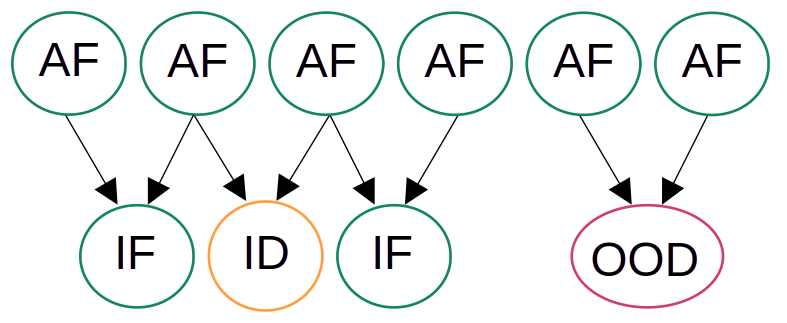
\includegraphics[width=0.45\textwidth, trim=0cm 0cm 0cm 0cm, clip]{IDvsOOD.png}
            \caption{
                \textbf{Conceptual difference between ID and OOD:} In-distribution \textbf{(ID, orange)} and Out-of-distribution \textbf{(OOD, red)} inferred facts are shown. All \textbf{green} components are seen during training, including all atomic facts \textbf{(AF)} and some inferred facts \textbf{(IF)}.
                %\textbf{Conceptual difference between In-distribution and Out-of-distribution:} All atomic facts (\textbf{AF}) are seen during training (top, \textbf{green}). In this example, inferred facts (bottom) are made from two atomic facts each ($\mathcal{F}_2$). In-distribution inferred facts (\textbf{ID}, \textbf{orange}) only use atomic facts that were used in inferred facts the model was trained on (\textbf{green}, \textbf{IF}). Out-of-distribution inferred facts (\textbf{OOD}, \textbf{red}) only use atomic facts that were not used in any inferred fact that the model was trained on.
                %As we omitted the underlying knowledge graph, note that the 2-hop deduction for every inferred fact must exist as a valid path $p_2$ in this graph. 
            }
            \label{fig:IDvsOOD}
        \end{figure}
        
        \begin{definition}[In-distribution vs.\ Out-of-distribution] $ $
            \label{def:id_ood}
            \newline\textbf{In-distribution (ID)}: An \textbf{inferred fact} derived from combinations of atomic facts that were \textbf{present in the training} data but never appeared together in this specific combination. The model \textbf{has seen} all knowledge components \textbf{separately} and different reasoning combinations involving them, but not in this particular test arrangement. 
            \newline\textbf{Out-of-distribution (OOD)}: An \textbf{inferred fact} derived from atomic facts that were \textbf{present in the training} data but \textbf{never used} in \textbf{any} train reasoning paths. The model has seen the individual knowledge components, but not how they should be applied in the context being tested.
            \newline\textbf{Figure \ref{fig:IDvsOOD}} shows trained facts (atomic and inferred) related to ID and OOD testing facts. 
        \end{definition}
        
        As we show in our experiments, \emph{OOD} queries can be especially challenging, requiring truly \emph{structural} generalization rather than partial memorization. This is precisely where sufficiently high \(\phi_r\) ratios become critical for enabling the Transformers’ \emph{grokking}-driven jump from local memorization to robust multi-hop reasoning.
        
    \subsection{Lemmas and Bounds}
        The first lemma we introduce makes clear that (1) picking nodes vs. arranging them in paths vs. the existence of edges leads to an asymptotic upper bound, and (2) even large KBs do not grow $\phi_{n,r}$ beyond roughly $b^{n-1}$ without additional data augmentation.

        \paragraph{Lemma 1 (Asymptotic Bound on the Number of $n$-hop Paths).}
            \label{lem:asymptoticF_n}
            \emph{Consider a knowledge base (KB) with $|\mathcal{V}|$ entities, average branching factor $b$, and an (approximate) random-graph assumption that each potential \emph{directed} edge between two distinct nodes is present with probability $\tfrac{b}{|\mathcal{V}|-1}$. Then, for large $|\mathcal{V}|$, the expected number of valid $n$-hop paths satisfies:}
            \[
            |\mathcal{F}_n| \;\approx\; \binom{|\mathcal{V}|}{n+1}\,(n+1)!\,
            \Bigl(\tfrac{b}{|\mathcal{V}|-1}\Bigr)^{\!n}.
            \]
            \emph{Moreover, in the limit $|\mathcal{V}|\to\infty$, the relation-specific ratio $\phi_{n,r}$ (i.e., the ratio of n-hop to 1-hop facts for relation r) remains bounded above by $b^{\,n-1}$.}
        
            For a \emph{Proof of Lemma 1} see Appendix \ref{sec:proof_lemma1}. For a lower generalization bound on the number of nodes $|\mathcal{V}|$, see Appendix \ref{sec:appendix_boundNlower}.           
            The second lemma makes clear that each relation’s branching factor $b_r$ must be sufficiently large to surpass the empirical threshold $\phi_G$. If one or more relations fall below that threshold, full generalization across \emph{all} relations will not occur -- even though partial generalization might emerge for the higher- $b_r$ relations.
            
        \paragraph{Lemma 2 (Necessary Condition for Full Generalizability).}
            \label{lem:phi_condition}
            \emph{Let $\phi_G$ be the minimal ratio required to trigger grokking-based generalization for a given model architecture. A KB is \textbf{fully generalizable} over $n$-hop facts only if $ \forall\,r\in\mathcal{R}$}
            \[ 
             \phi_{n,r} 
            \;\geq\; 
            \phi_G 
            \quad\Rightarrow\quad
            b_r 
            \;>\; 
            \sqrt[n-1]{\frac{\phi_G\,|\mathcal{V}|\,(|\mathcal{V}|-1)^{n}}{\binom{|\mathcal{V}|}{n+1}\,(n+1)!}},
            \]
            \emph{where $b_r=\frac{|\mathcal{F}_{A,r}|}{|\mathcal{V}|}$ is the relation-specific branching factor. Equivalently, if any $b_r$ falls below this threshold, the KB cannot be fully generalizable.}

            For a \emph{Sketch of Proof of Lemma 2} see Appendix \ref{sec:proof_lemma2}. 
            
            \begin{table}[t]
            \centering
            \caption{\textbf{Key Notation Table.} Frequently used symbols throughout this paper.}
            \vskip 0.1in
            \label{tab:key_notation}
            \begin{adjustbox}{max width=0.49\textwidth}
                \begin{tabular}{r l}
                    \toprule
                    \textbf{Symbol} & \textbf{Meaning} \\
                    \midrule
                    \(\mathcal{V}\) & Set of entities (nodes) in the KG \\
                    \(\mathcal{R}\) & Set of relation types (edges) \\
                    \(\mathcal{F}_A\) & Atomic facts (1-hop) \(\subseteq \mathcal{V}\times\mathcal{R}\times\mathcal{V}\)\\
                    \(\mathcal{F}_I\) & Inferred facts (multi-hop) \(\bigcup_{n\ge2}\mathcal{F}_n\)\\
                    \(b\) & Average branching factor \(\tfrac{|\mathcal{F}_A|}{|\mathcal{V}|}\) \\
                    \(\phi_r\) & \(\tfrac{|\mathcal{F}_{I,r}|}{|\mathcal{F}_{A,r}|}\) (ratio of inferred to atomic facts)\\
                    \(\phi_G\) & Minimal generalization ratio for successful grokking \\
                    \(I(h,r)\) & Inference step: from entity \(h\) via relation \(r\) to a neighbor \\
                    \bottomrule
                \end{tabular}
            \end{adjustbox}
            \end{table}
        